\documentclass[10pt, a4paper]{article}
\usepackage{latexsym}
\usepackage{amssymb,amsmath}
\usepackage[pdftex]{graphicx}
\newcommand{\dbar}[1]{\Bar{\Bar{#1}}}

\topmargin = 0.1in \textwidth=5.7in \textheight=8.6in

\oddsidemargin = 0.1in \evensidemargin= 0.1in

% headers
\usepackage{fancyhdr}
\usepackage{bm}
\usepackage{subfigmat}
\usepackage{longtable}
\usepackage{booktabs}
\pagestyle{fancy}
\chead{} 
\rhead{\thepage} 
% footer
\lfoot{\small\scshape } 
\cfoot{} 
%%%% insert your name here %%%%
\rfoot{\footnotesize Burton} 
\renewcommand{\headrulewidth}{.3pt} 
\renewcommand{\footrulewidth}{.3pt}
\setlength\voffset{-0.25in}
\setlength\textheight{648pt}

\begin{document}

\title{Weissinger Vortex Lifting Line as a GP}
\author{Michael Burton}
\maketitle

This write-up is an attempt to formulate the Weissinger Vortex Lifting Line method as a geometric program (GP).  
With little modification this method can be cast as a signomial program (SP).  
However, formulation as a GP is not as straightforward.  
This write-up attempts to explain why this method is not GP-compatible even though it is convex. 
One approach to formulate this method as a GP is presented so that new insights might be had in solving this problem. 

\section*{Weissinger Vortex Lifting Line}

The Weissinger Vortex Lifting Line (WVL) is a lifting line method used to predict aerodynamic forces on a lifting surface.  It uses a collection of horseshoe vortex filaments along the span, each h.v.\ filament having constant strength $\Gamma_i$. 
A derivation of the WVL will not be given in this write-up as it is well documented elsewhere and follows the same principles of a vortex lattice method. 
The equations for the parameters of interest, coefficient of lift $C_L$, and coefficient of induced drag $C_{D_i}$, are 

\begin{align}
    \label{e:cl}
    C_L &= 2 \bar{\Gamma}^{\mathrm{T}} (\bar{V}_x \vec{\Delta y})/S_{\mathrm{ref}} \\
    &= \frac{2}{S_{\mathrm{ref}}} (\bar{\Gamma}_1 \bar{V}_{x_1} \Delta y_1 + \bar{\Gamma}_2 \bar{V}_{x_2} \Delta y_2 + \cdots + \bar{\Gamma}_N \bar{V}_{x_N} \Delta y_N) \nonumber \\
    \label{e:cdi}
    C_{D_i} &= 2 \bar{\Gamma}^{\mathrm{T}} \bar{\bar{B}} \bar{\Gamma}/S_{\mathrm{ref}} \\
            &= \frac{2}{S_{\mathrm{ref}}} (B_{1,1} \Gamma_1^2 + B_{1,2} \Gamma_1 \Gamma_2 + B_{1,3}\Gamma_1 \Gamma_3 + \cdots + B_{N,N} \Gamma_N^2) \nonumber
\end{align}
where the normalized h.v.\ filament strength is $ \bar{\Gamma} = \Gamma/V_{\inf}$, and the local normalized x-component of the velocity is $\bar{V}_x = u/V_{\inf}$.
The h.v.\ filaments can be distributed along the span in a cosine distribution as shown in Figure~\ref{f:wvl}.  

\begin{figure}[h!]
	\begin{center}
	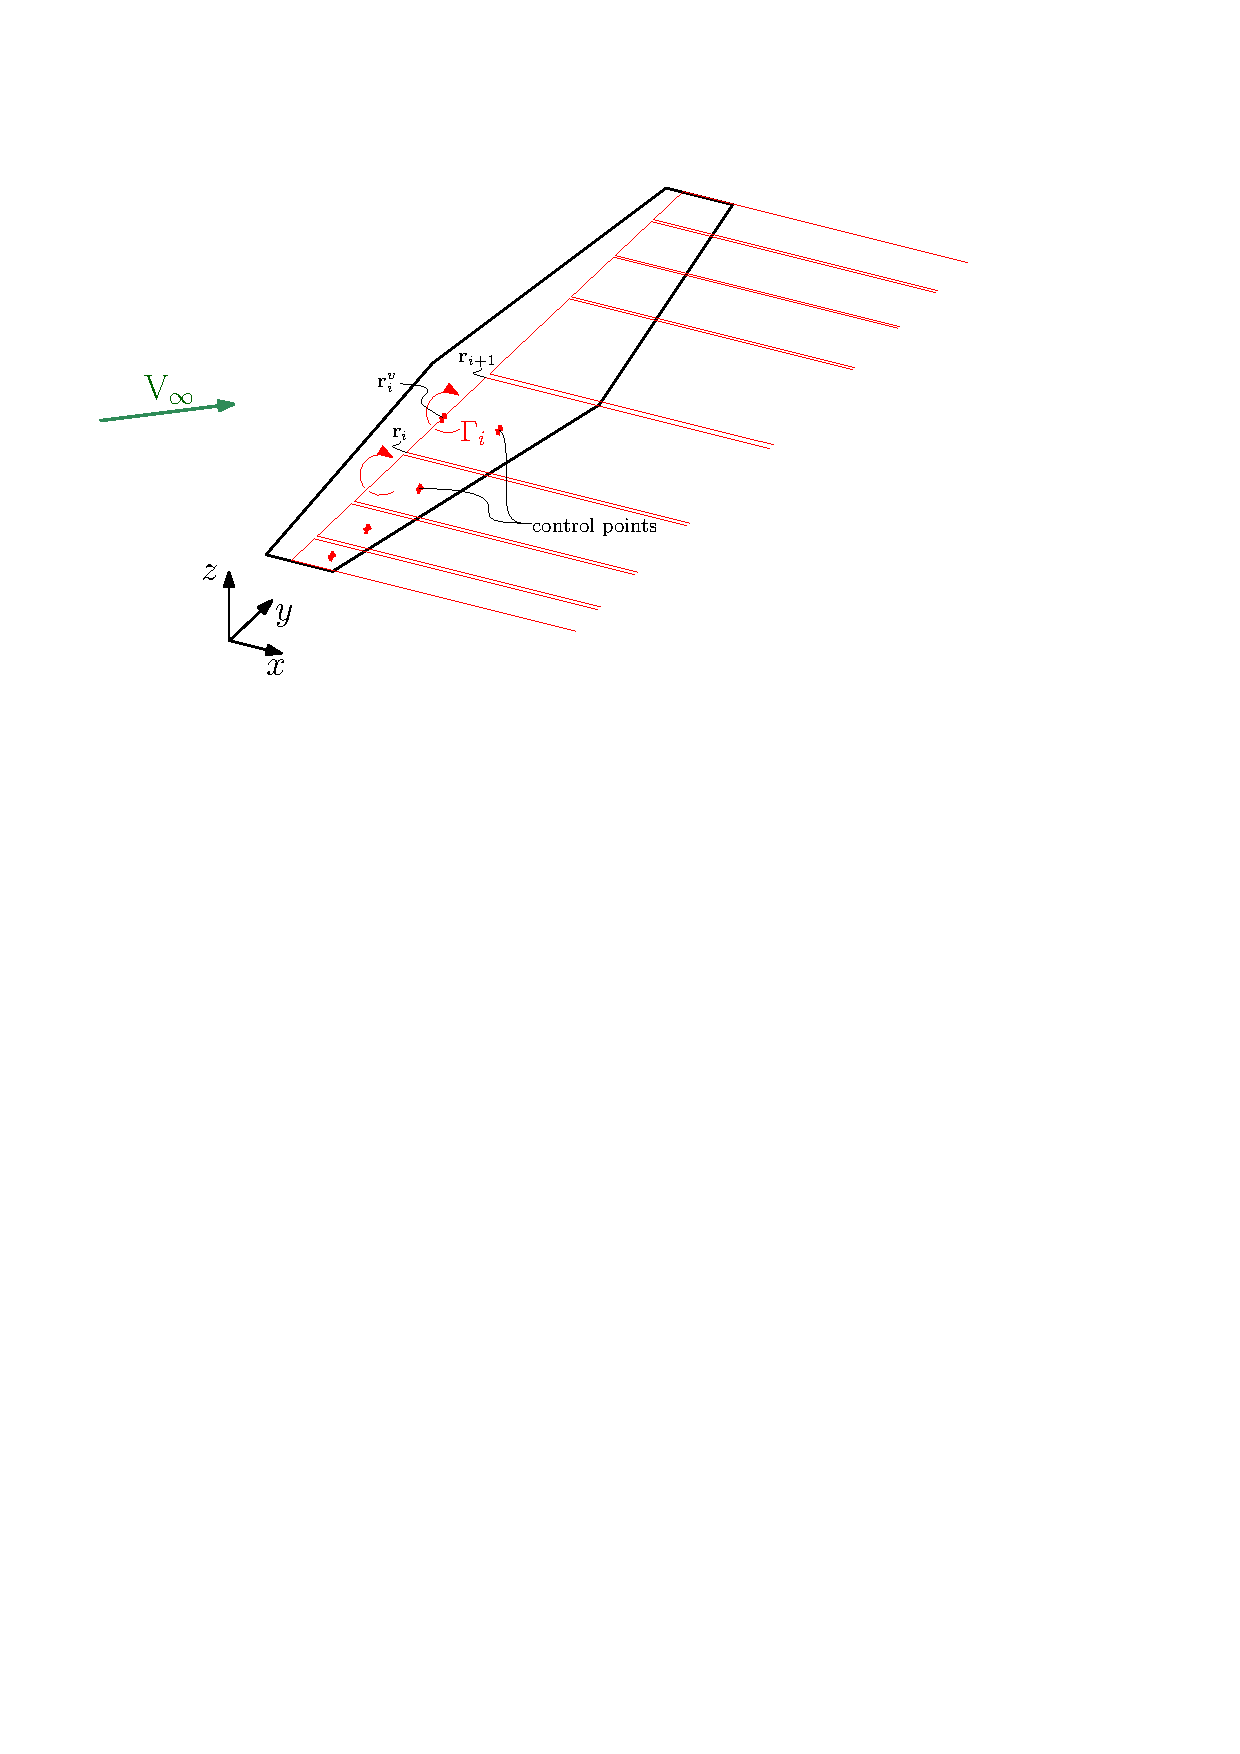
\includegraphics[width=0.8\textwidth]{wvl.pdf}
    \caption{Cosine distribution of h.v.\ filaments on constant taper wing.}
\label{f:wvl}
\end{center}
\end{figure}

The h.v.\ filament strength $\Gamma$, is related to the physical geometry through the Aerodynamic Influence Coefficient (AIC) matrix $\bar{\bar{A}}$, 

\begin{equation}
    \bar{\bar{A}} \bar{\Gamma} = \bar{\mathbf{U}}
\end{equation}
where $\bar{\mathbf{U}}$ is the local normalized velocity vector. The AIC matrix is defined as 

\begin{align}
    A_{ij} &\equiv \hat{\mathbf{V}}_j (\mathbf{r}_i^c) \cdot \bm{n}_{0_i} \\
    \hat{\mathbf{V}}_i (\mathbf{r}) &= \frac{1}{4\pi} \left[ \frac{\mathbf{a} \times \mathbf{b}}{|\mathbf{a}| |\mathbf{b}| + \mathbf{a} \cdot \mathbf{b}} \left( \frac{1}{|\mathbf{a}|} + \frac{1}{|\mathbf{b}|}\right) + \frac{\mathbf{a} \times \hat{\mathbf{x}}}{|\mathbf{a}| - \mathbf{a} \cdot \hat{\mathbf{x}}} \frac{1}{|\mathbf{a}|} - \frac{\mathbf{b} \times \hat{\mathbf{x}}}{|\mathbf{b}| - \mathbf{b} \cdot \hat{\mathbf{x}}} \frac{1}{|\mathbf{b}|} \right]
\end{align}

where the vectors $\bm{\mathrm{a}}$, $\bm{\mathrm{b}}$, and $\bm{\mathrm{x}}$ are defined in Figure~\ref{f:singlehv}. The control vector $\bm{\mathrm{r}}_i^c$ is defined in Figure~\ref{f:singlecp}. 
The WVL method assumes the control vector $\bm{\mathrm{r}}_i^c$ to be a vector to the three-quarters chord $\frac{3}{4}c$.  
The unit normal vector $\bm{n}_{0_i}$, can be approximated as a function of the local twist

\begin{equation}
    \bm{n}_{0_i} \approx \sin{\theta_i} \hat{x} + \cos{\theta_i} \hat{z}
\end{equation}

\begin{figure}[h!]
 \begin{subfigmatrix}{2}% number of columns
\subfigure[$\bm{\mathrm{a}}$, $\bm{\mathrm{b}}$, and $\bm{\mathrm{x}}$ vector definition\label{f:singlehv}]{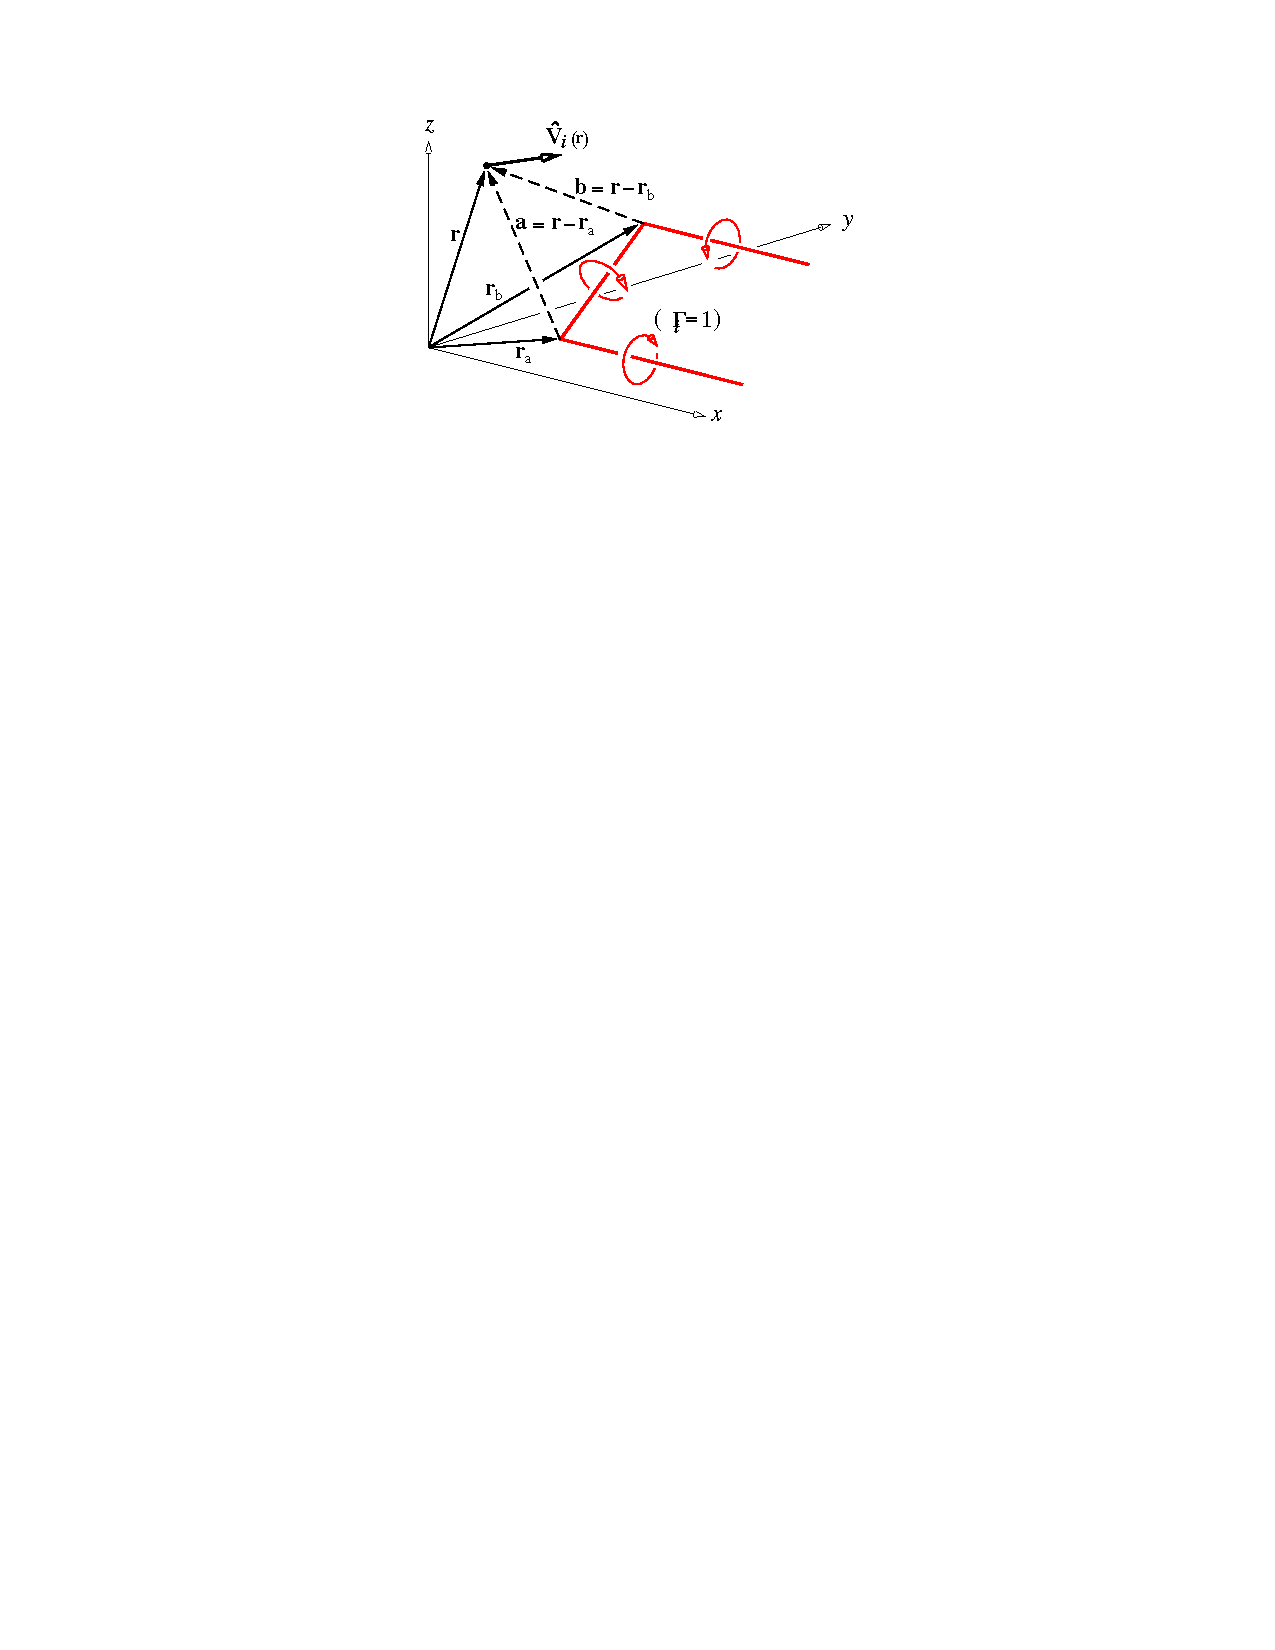
\includegraphics{singlehv.pdf}}
\subfigure[Control vector $\bm{\mathrm{r}}_i^c$ definition\label{f:singlecp}]{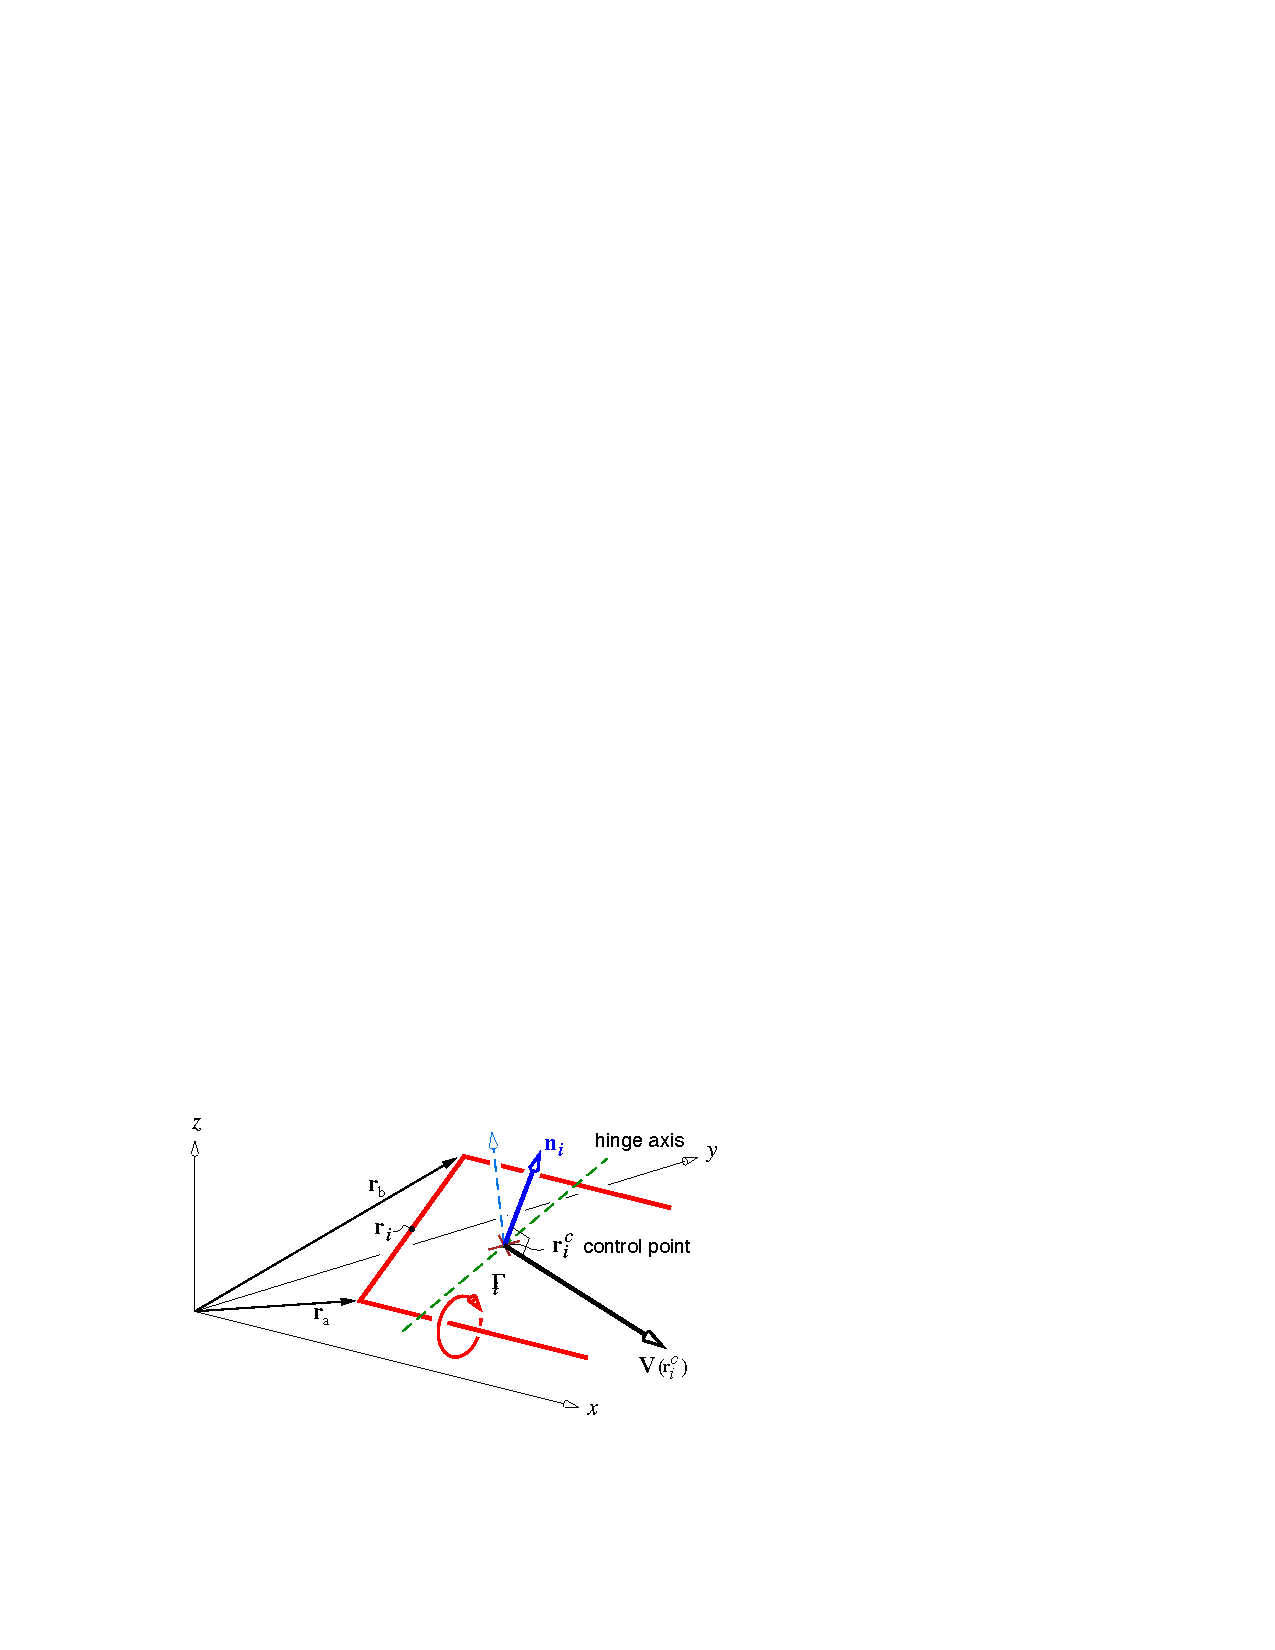
\includegraphics{singlecp.pdf}}
 \end{subfigmatrix}
 \caption{Geometry of one horseshoe vortex.}
\label{f:singlevortex}
\end{figure}

The $\bar{\bar{B}}$ matrix, also a function of the geometry, depends on the vortex midpoint $\mathbf{r}_i^v$, not the control point $\mathbf{r}_i^c$

\begin{align}
    B_{ij} &= \frac{\Delta y_i}{4\pi} \left[ \frac{y_i^v - y_i}{{(y_i^v - y_i)}^2 + {(z_i^v - z_i)}^2} - \frac{y_i^v - y_{i+1}}{{(y_i^v - y_{i+1})}^2 + {(z_i^v - z_{i+1})}^2} \right] \\
    &+ \frac{\Delta z_i}{4\pi} \left[ \frac{z_i^v - y_i}{{(z_i^v - y_i)}^2 + {(z_i^v - z_i)}^2} - \frac{z_i^v - z_{i+1}}{{(y_i^v - y_{i+1})}^2 + {(z_i^v - z_{i+1})}^2} \right] \nonumber
\end{align}

The system of equations can be solved using a Newton method and by specifying flow conditions such as a specified lift coefficient $C_{L_{\mathrm{spec}}}$.

% \begin{figure}[h!]
% 	\begin{center}
% 	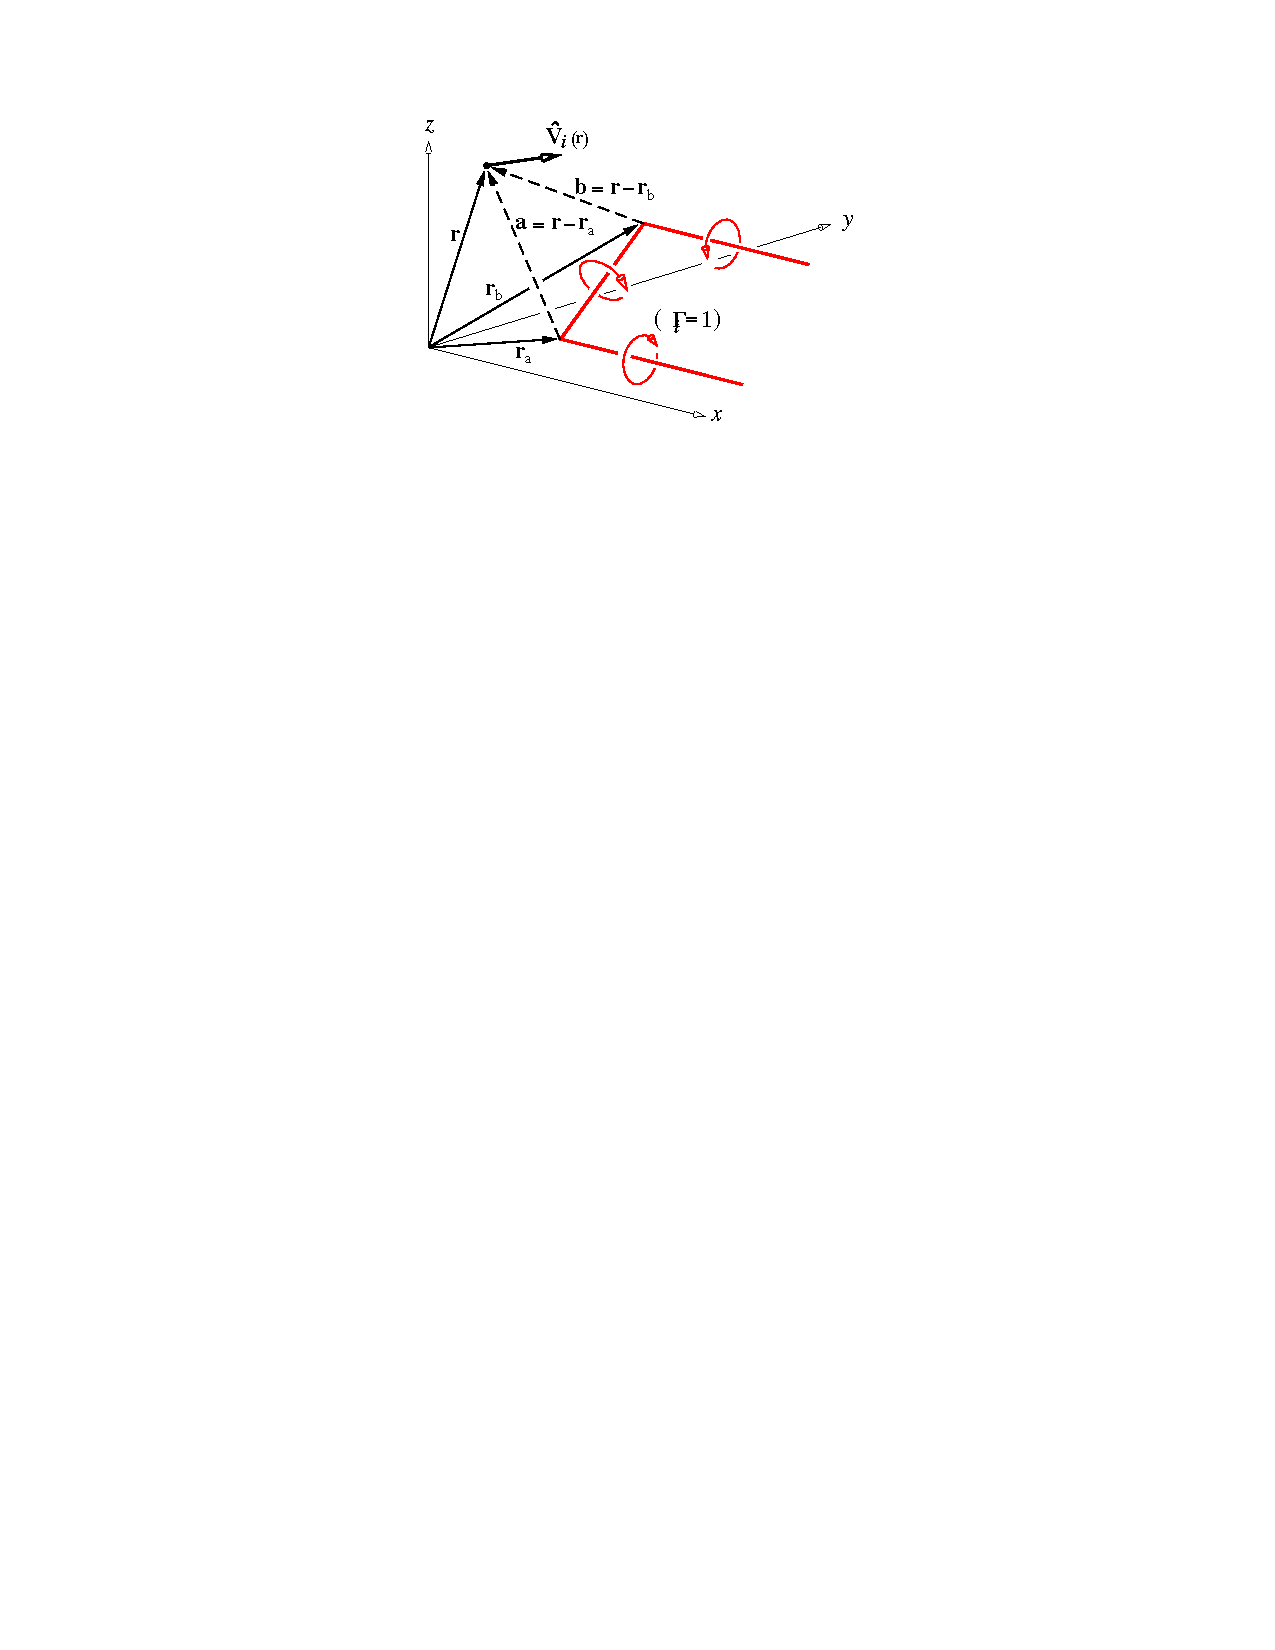
\includegraphics[width=0.6\textwidth]{singlehv.pdf}
%     \caption{Geometry of one horseshoe vortex.}
% 	\label{f:singlehv}
% 	\end{center}
% \end{figure}

\section*{WVL as a GP:\ Problem Set Up}

Geometric programs are non-linear optimization problems with a particular form

\begin{alignat*}{3}
    \text{minimize }\quad & g_0 (x) && \\
    \text{subject to }\quad & f_i(x) &= 1,\quad  i&=1,\dots,m \\
                            & g_i(x) &\leq 1, \quad i&=1,\dots,n 
\end{alignat*}
where monomials $f(x)$ and posynomials $g(x)$ are defined as

\begin{align}
    f(x) &= cx_1^{a_1}x_2^{a_2}  \dots x_n^{a_n}  \\
    g(x) &= \sum_{k=1}^K c_k x_1^{a_1k}x_2^{a_2k}  \dots x_n^{a_nk}
\end{align}

For the purposes of this exercise, it is assumed that the geometry is known.  
Specifically, all control vectors $\mathbf{r}_i^c$, node vectors $\mathbf{r}_i$, and midpoint vectors $\mathbf{r}_i^v$ are known.  Thus the AIC matrix $\bar{\bar{A}}$, and the $\bar{\bar{B}}$ matrix are also known.  
Furthermore, we will assume for now that $V_{x_i} = V_{\infty}$.  
Finally, the lift coefficient $C_L$, will be constrained by a specified number $C_{L_{\mathrm{spec}}}$, and the drag coefficient $C_{D_i}$, will be minimized.
This simplifies Equations~\ref{e:cl} and~\ref{e:cdi} to 

\begin{align}
    \label{e:clsp}
    C_{L_{\mathrm{spec}}} &= 2 \bar{\Gamma}^{\mathrm{T}} (\vec{\Delta y})/S_{\mathrm{ref}} \\
    \label{e:cdsp}
    C_{D_i} &= 2 \bar{\Gamma}^{\mathrm{T}} \bar{\bar{B}} \bar{\Gamma}/S_{\mathrm{ref}} 
\end{align}
Because the geometry is known, this problem can be adequately defined by these two equations. 

At first glance, Equations~\ref{e:clsp} and~\ref{e:cdsp} both seem like posynomials.  
If this were the case, the problem would be solved and we could stop here.  
However, a closer look at the upper and lower variable bounds reveals this is not the case. 

For a GP to be well defined, each variable must have an upper or lower bound.
A variable with a value, is called a fixed variable and bounded by the assigned value.  
A maximized variable is lower bounded by the objective function and a minimized variable is upper bounded by the objective function. 
Every other variable must be upper and lower bounded by the constraints and direction of the inequalities.  

Because $C_{D_i}$ is being minimized and $C_{L_{\mathrm{spec}}}$ and $\bar{\bar{B}}$ are known, the only direction of inequalities that adequately upper and lower bound each variable is

\begin{align}
    \text{minimize} & \quad C_{D_i} \nonumber \\
    \label{e:cleq}
    C_{L_{\mathrm{spec}}} &\leq 2 \bar{\Gamma}^{\mathrm{T}} (\vec{\Delta y})/S_{\mathrm{ref}} \\
    \label{e:cdeq}
    C_{D_i} &\geq 2 \bar{\Gamma}^{\mathrm{T}} \bar{\bar{B}} \bar{\Gamma}/S_{\mathrm{ref}}.
\end{align}
Table~\ref{t:bounds} shows every variable and lists its upper and lower bounds. 

\begin{longtable}{lcc}
\caption{Variable Boundedness}\\
\toprule
\toprule
\label{t:bounds}
Variable                    & Upper Bound       & Lower Bound      \\ \midrule
$C_{L_{\mathrm{spec}}}$     & Value             & Value            \\
$C_{D_i}$                   & Objective         & Eq.~\ref{e:cdeq} \\
$\bar{\Gamma}_i$            & Eq.~\ref{e:cdeq}  & Eq.~\ref{e:cleq} \\
$B_{ij}$                    & Value             & Value            \\
$S_{\mathrm{ref}}$          & Value             & Value            \\
\bottomrule
\end{longtable}

Unfortunately, this formulation is not GP-compatible because Equation~\ref{e:cleq} is not posynomial.  
A general rule of thumb for GP compatibility is that sums of ``bad'' things are GP compatible and sums of ``good'' things are not.  
For example, weight is usually a bad thing for aircraft.  Therefore, a weight summation $W_{\mathrm{total}} \geq \sum W_i$, is usually GP compatible. 
In this case, we have multiple h.v.\ filaments that each provide some lift.  
From a very simplistic standpoint, the solver cannot correctly optimize the $\Gamma$ values because it only sees each $\Gamma$ as wanting more because lift is a good thing. 

\subsection*{WVL as an SP}

While the GP formulation of the WVL method previously discussed is not GP-compatible, it can be written as a signomial program (SP).  SPs have the form

\begin{alignat*}{3}
    \text{minimize }\quad & g_0 (x) && \\
    \text{subject to }\quad & f_i(x) &= 1,\quad  i&=1,\dots,m \\
                            & g_i(x) &- h_i(x) \leq 1, \quad i&=1,\dots,n 
\end{alignat*}
where each $f$ is a monomial and each $g$ and $h$ is a posynomial. SPs solves a difference of convex problems and requires multiple GP solutions.  Because it is a difference of convex, the solution is not guaranteed to be optimal.  Thus, the SP formulation of the WVL may be useful but is less desirable because of the increased solve time and decreased reliability. 

Both Equations~\ref{e:cleq} and~\ref{e:cdeq} are SP.  It is worth noting here that the $\bar{\bar{B}}$ matrix is positive along the diagonal and negative everywhere else

\begin{equation*}
    \bar{\bar{B}} =  
    \begin{bmatrix} 
        + & - & - & \dots & - \\
        - & + & - & \dots & - \\
        - & - & + & \dots & - \\
        \vdots & \vdots & \vdots & \ddots & \vdots \\
        - & - & - & \dots & + 
    \end{bmatrix}
\end{equation*}
The $\bar{\bar{B}}$ matrix can be broken into its diagonal and off-diagonal components 

\begin{equation}
    \bar{\bar{B}} = \bar{\bar{B}}_{\mathrm{diag}} + \bar{\bar{B}}_{\mathrm{offd}}
\end{equation}
where

\begin{equation*}
    \bar{\bar{B}}_{\mathrm{diag}} =  
    \begin{bmatrix} 
        B_{11} & 0 & 0 & \dots & 0 \\
        0 & B_{22} & 0 & \dots & 0 \\
        0 & 0 & B_{33} & \dots & 0 \\
        \vdots & \vdots & \vdots & \ddots & \vdots \\
        0 & 0 & 0 & \dots & B_{NN}
    \end{bmatrix} \quad
    \bar{\bar{B}}_{\mathrm{offd}} =  
    \begin{bmatrix} 
        0      & B_{12} & B_{13} & \dots  & B_{1N} \\
        B_{21} & 0      & B_{23} & \dots  & B_{2N} \\
        B_{31} & B_{32} & 0      & \dots  & B_{3N} \\
        \vdots & \vdots & \vdots & \ddots & \vdots \\
        B_{N1} & B_{N2} & B_{N3} & \dots  & 0
    \end{bmatrix} \quad
\end{equation*}

Using this breakdown of $\bar{\bar{B}}$ Equation~\ref{e:cdeq} can be rewritten as

\begin{equation}
    C_{D_i} + 2\bar{\Gamma}^{\mathrm{T}} \bar{\bar{B}}_{\mathrm{offd}} \bar{\Gamma}/S_{\mathrm{ref}} \geq 2 \bar{\Gamma}^{\mathrm{T}} \bar{\bar{B}}_{\mathrm{diag}} \bar{\Gamma}/S_{\mathrm{ref}}.
\end{equation}
so that each variable is positive. This forumlation can be solved as a SP.  An example case of constant taper wing described in Figure~\ref{f:samplewing} was solved as an SP.

\begin{figure}[h!]
	\begin{center}
	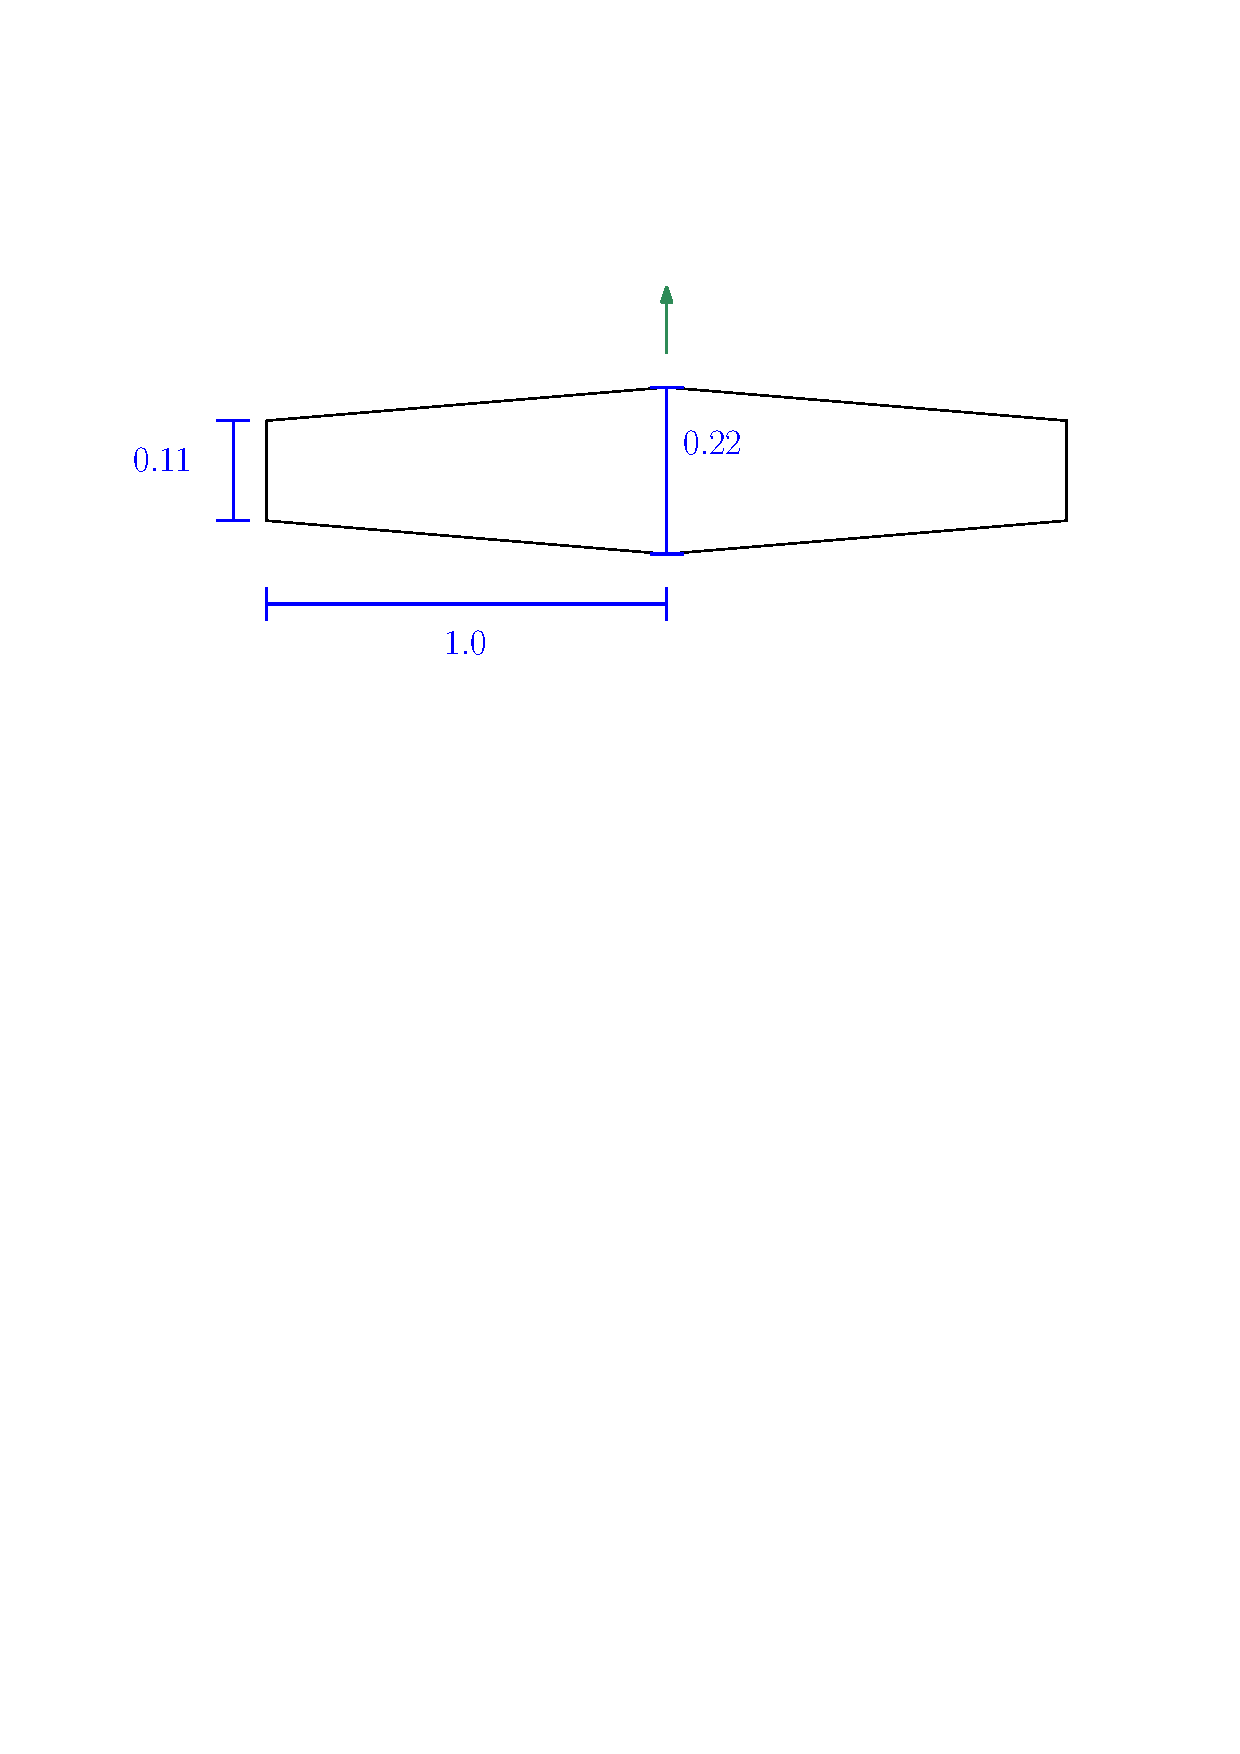
\includegraphics[width=0.8\textwidth]{samplewing.pdf}
    \caption{Sample wing used for comparison between SP model and numerical solution using a Newton method.}
\label{f:samplewing}
\end{center}
\end{figure}

The lifting distribution and induced drag were evaluated using a Newton method implementation of the WVL. This solution was compared to the SP solution using 6 h.v.\ filaments. 
The flight conditions are: $C_{L_{\mathrm{spec}}} = 1.1$, zero side slip and zero roll.  
The comparison between $\Gamma$ and $C_{D_i}$ is shown in Table~\ref{t:spcomp}.
Only the first three $\Gamma$ values are shown because the steady level flight condition means the three h.v.\ filaments on the other side of the wing have the same value.  

\begin{longtable}{lccc}
\caption{WVL Method Comparison}\\
\toprule
\toprule
\label{t:spcomp}
Variable            & Newton Method     & SP Model  & Error  \\ \midrule
$C_{D_i} \quad (N=6)$& 0.027             & 0.0263    & 3.0\%  \\
$\bar{\Gamma}_1$    & 0.0565            & 0.0432    & 23\%   \\
$\bar{\Gamma}_2$    & 0.0824            & 0.0850    & 3.2\%  \\
$\bar{\Gamma}_3$    & 0.1070            & 0.1086    & 1.5\%  \\
$C_{D_i} \quad (N=20)$& 0.0307            & 0.0302    & 1.8\%  \\
\bottomrule
\end{longtable}

This comparison shows that the SP model captures the correct trends but is not as accurate as the Newton method.  The SP model solved in 0.15 seconds and took 7 GP solves.  Increasing the number of h.v. filaments to 20 decreases the error, but is still not as accurate.  With $N=20$, the SP model solved in 0.885 seconds and took 15 GP solves. 
 
\section*{Possible GP Formulation}

This section aims to propose one solution that may allow for a GP-compatible way to write the WVL.  This formulation is not complete. 

Let's assume that the strength of each h.v.\ filament multiplied by the length that it spans is equal, 

\begin{equation}
    x_{C_L} = \bar{\Gamma}_1 \Delta y_1 = \bar{\Gamma}_2 \Delta y_2 = \cdots = \bar{\Gamma}_N \Delta y_N.
\end{equation}
If this can be true, then Equation~\ref{e:cleq} can be rewritten as

\begin{equation}
    C_{L_{\mathrm{spec}}} \leq 2Nx_{C_L}/S_{\mathrm{ref}}
\end{equation}
which is GP-compatible. 

The other roadblock to GP-compatibility is that the off diagonals of the $\bar{\bar{B}}$ matrix are negative. This can be solved by using a different distribution of h.v.\ filaments that are centered around the center of the wing as shown in Figure~\ref{f:gp_form}.
Under this distribution the $\bar{\bar{B}}$ matrix is strictly positive.  
This distribution of h.v.\ filaments is valid and can be solved with a Newton method in the same way as the distribution previously described. 
\pagebreak
\begin{figure}[h!]
	\begin{center}
	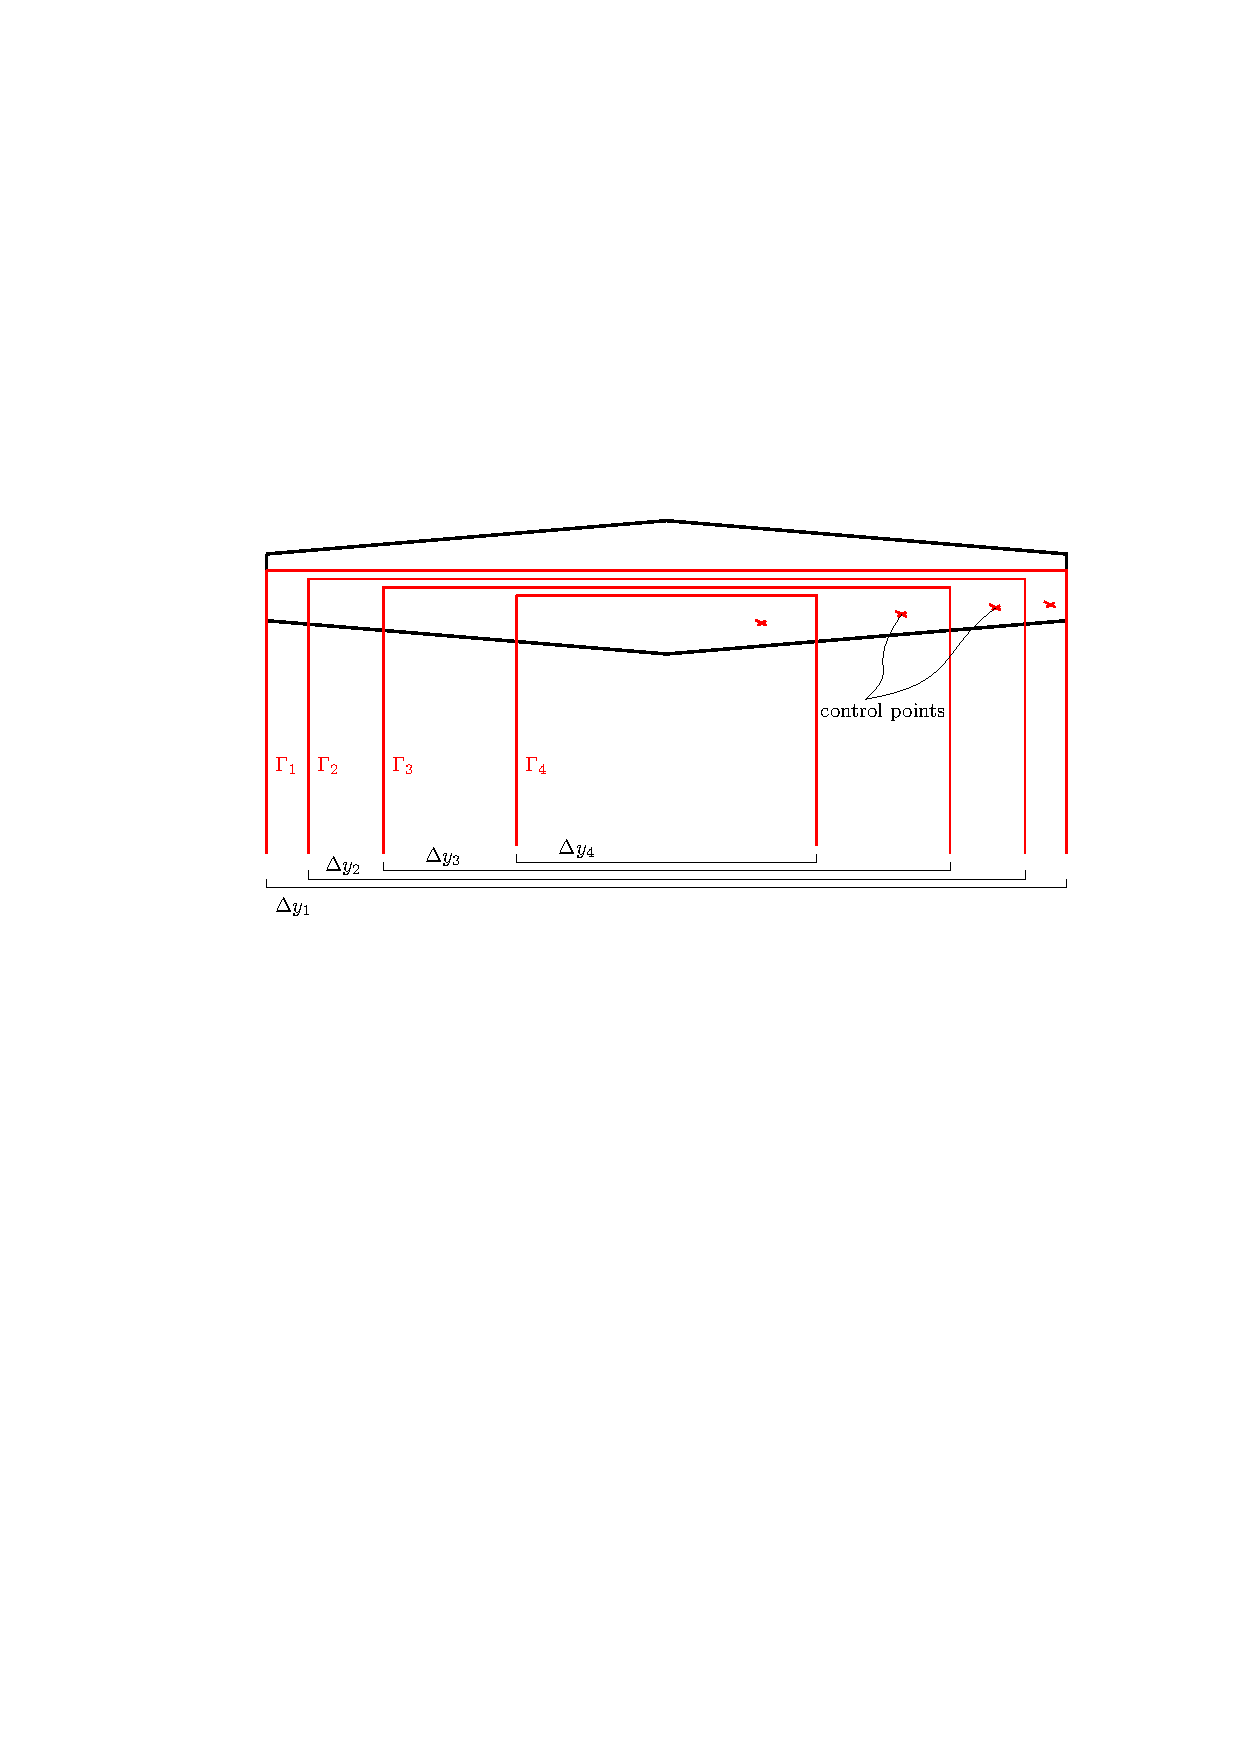
\includegraphics[width=0.8\textwidth]{gp_form.pdf}
    \caption{Distribution of spanwise vorticies centered on center of wing.}
\label{f:gp_form}
\end{center}
\end{figure}

However, because $\Delta y$ needs to be optimized with $\Gamma$, the distribution of h.v.\ filaments is not known beforehand, only that they are centered on the middle of the wing.  
This means that the $\bar{\bar{B}}$ matrix cannot be specified apriori but must be solved for in the optimization.  

Let's begin with a simple example and assume that the wing has no dihedral.  Because the vortex midpoints will all be in the same place at $y=0$, the $\bar{\bar{B}}$ matrix simplifies nicely to

\begin{equation}
    B_{ij} = \frac{1}{\pi} \frac{\Delta y_j}{\Delta y_i}
\end{equation}

Thus, the GP formulation under these assumptions is

\begin{align}
    \text{minimize} & \quad C_{D_i} \nonumber \\
    C_{L_{\mathrm{spec}}} &\leq 2 N x_{C_L}/S_{\mathrm{ref}} \\
    x_{C_L} &= \bar{\Gamma} \vec{\Delta y} \\
    C_{D_i} &\geq 2 \bar{\Gamma}^{\mathrm{T}} \bar{\bar{B}} \bar{\Gamma}/S_{\mathrm{ref}} \\
    \label{e:bij}
    B_{ij} &\geq \frac{1}{\pi} \frac{\Delta y_j}{\Delta y_i}.
\end{align}
Each variable is bounded as before.  However, $N$ new variables exist in $\vec{\Delta y}$ that are all upper unbounded.  Unfortunately, because each $\Delta y_i$ appears in both the numerator and denominator of Equation~\ref{e:bij}, the upper bound is negated in this equation. 

And this is where I hit a wall.  I don't know how to correctly upper bound $\Delta y$. There may be a way to upper bound $\Delta y$ with $S_{\mathrm{ref}}$, but I haven't found a way to do it.  I appreciate any and all ideas you may have to solving this problem or presenting a different formulation that is GP-compatible. 

\end{document}
